%%This is a very basic article template.
%%There is just one section and two subsections.
\documentclass{article}
\usepackage{graphicx}
\usepackage{cite}
\usepackage{booktabs}
\graphicspath{ {images/} }


\begin{document}

\bibliographystyle{plain}


\section{Title}

\subsection{Introduction}
%introduce whole study and paper here (together)

\subsection{Background}
%literature background (Natalie)

\subsection{Materials and Methods}


The original dataset utilised in this study consists in 1,562 responses from a
quantitative survey conducted on behalf of the ACNC by ChantLink in 2013. It
does not include a pilot phase of 62 responses. The survey collected information
about levels of trust in charities and factors that may affect these levels. The
respondents were asked to rate their level of trust and their agreement with a
series of statements about charities on a scale from 1 to 10. They also were
asked about their involvement, knowledge of charities sector and demographics.
Specifically, the survey was divided into 5 sections: Awareness and Involvement
in Charities, Trust, Regulation, Public Register of Charities and Demographics.

Aiming to cluster the survey respondents according their trust and confidence in
charities, a new dataset was obtained from the original dataset. It consists of
the Trust section responses which were rated on the scale from 1 to 10. In
addition, the questions not answered by all the respondents and those with
user-typed responses were removed. This procedure was adopted in order to select
informative and comparable questions as the survey contains different types of
questions. Overall, 1,562 responses of 43 different questions was considered in
the clustering step.

Since the dataset can be represented as a graph, the methodology utilised for
clustering is based on a novel graph-based clustering algorithm propose by
~\cite{Inostroza2008}. The MSTkNN combines a Minimum Spanning Tree (MST) and a
k-Nearest Neighbor (kNN) proximity graphs. This combination allows us to perform
a graph partitioning operation, which produce a clustering of the dataset
represented by its graph. The graph partitioning separates the data in groups
with similar characteristics utilizing a given proximity measurement. In this
case, the Spearman correlation was used to measure the distance between
different features of the dataset's graph.

Given a undirected and connected graph, a MST is a subgraph which is a tree and
contain all the objects connected by the minimum possible distance between each
other, based on a determined measurement of the distance. Whereas, the kNN graph
is a graph where their objects are connected if they are commutual k nearest
neighbors of each other according to a defined value of k. In this work, the
value of k was defined as 3 for computing the kNN graph. The merge of these
methods permit delete the connection between two objects in the MST if they are
not reciprocally one of the k nearest of each other. Consequently, the MST is
partitioned into smaller subgraphs which are the resultant clusters.

%Normalization by row?


After clustering the dataset, the new score introduced by~\cite{Marsden2013}
was computed to highlight the individual characteristics of each cluster. The
CM1 scores gives a overview about differences in averages for each feature from
a specific cluster in the investigated dataset. The rank of the CM1 scores of a
cluster can be split into top or bottom features. The top features refers to
features whose average are greater in a specific cluster than in all the others,
while bottom refers to features whose average are less in a specific cluster
than in all the others. The CM1 scores are then computed using the following
formula~(\ref{eq:01}).

\begin{equation}
CM1(w,X,Y) = \frac{\frac{1}{\left|X\right|}  \sum_{x \in X} x_{w} - \frac{1}{\left|Y\right|}  \sum_{y \in Y} y_{w}} {1 + max_{y \in Y } \left\{ y_{w} \right\}- min_{y \in Y} \left\{y_{w}\right\} } \label{eq:01}
\end{equation}

%this study was based on the study done in UK and NZ


\subsection{Results}

The MSTkNN clustering algorithm was able to find 7 different clusters of
different sizes according Figure \ref{fig:Clusters}. These included Cluster0
(13\%), Cluster1 (10\%), Cluster2 (12\%), Cluster3 (20\%), Cluster4 (3\%),
Cluster5(36\%) and Cluster6 (6\%).


\begin{figure}[h]
	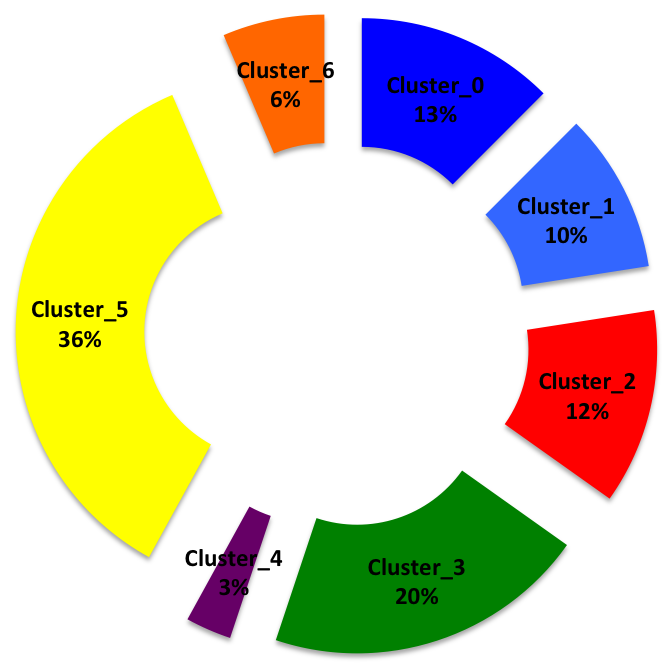
\includegraphics[ width=\textwidth ]{Clusters.png}
	\caption{\textbf{Percentage of respondents for each cluster discovered by the
	MSTkNN clustering algorithm} The MSTkNN.}
	\label{fig:Clusters}
\end{figure}

The CM1 score was calculated for all the 43 questions of the new dataset
for each of the discovered clusters. The selected top and bottom features for
each cluster is presented in the Tables~\ref{tab:top} and ~\ref{tab:bottom}.

% Table generated by Excel2LaTeX from sheet 'Sheet1'
\begin{table}[htbp]
  \centering
  \caption{Top features for each cluster (presented in descending order of
  score)}
    \begin{tabular}{rrrrrrr}
    \toprule
    Cluster\_0 & Cluster\_1 & Cluster\_2 & Cluster\_3 & Cluster\_4 & Cluster\_5 & Cluster6 \\
    \midrule
    Q11\_1\_1 & Q11\_4\_1 & Q11\_4\_1 & Q9\_19 & Q7B\_4 & Q9\_12 & Q7B\_1 \\
    Q9\_07 & Q11\_2\_1 & Q11\_1\_1 & Q9\_03 & Q11\_2\_1 & Q9\_08 & Q7B\_9 \\
    Q11\_6\_1 & Q11\_1\_1 & Q9\_20 & Q7A   & Q7B\_3 & Q9\_01 & Q7B\_8 \\
    Q9\_25 & Q11\_6\_1 & Q9\_21 & Q7B\_11 & Q9\_02 & Q9\_16 & Q9\_10 \\
    Q9\_22 & Q11\_3\_1 & Q11\_6\_1 & Q7B\_7 & Q9\_10 & Q9\_11 & Q7B\_10 \\
    Q9\_05 & Q11\_5\_1 & Q11\_3\_1 & Q9\_09 & Q11\_1\_1 & Q9\_03 & Q7B\_2 \\
    Q11\_3\_1 & Q9\_20 & Q11\_5\_1 & Q9\_10 & Q11\_4\_1 & Q9\_19 & Q7B\_5 \\
    Q9\_06 & Q9\_21 & Q9\_06 & Q9\_02 & Q11\_5\_1 & Q9\_13 & Q7B\_7 \\
    Q11\_5\_1 & Q9\_05 & Q9\_05 &       &       & Q9\_14 & Q9\_02 \\
    Q9\_24 & Q9\_06 & Q9\_07 &       &       &       & Q7B\_3 \\
    Q9\_20 & Q9\_07 &       &       &       &       & Q7B\_11 \\
    Q9\_23 &       &       &       &       &       & Q7B\_6 \\
    Q9\_21 &       &       &       &       &       & Q7B\_4 \\
    \bottomrule
    \end{tabular}
  \label{tab:top}
\end{table}

% Table generated by Excel2LaTeX from sheet 'Sheet2'
\begin{table}[htbp]
  \centering
  \caption{Bottom features for each cluster (presented in descending order of
  score)}
    \begin{tabular}{rrrrrrr}
    \toprule
    Cluster\_0 & Cluster\_1 & Cluster\_2 & Cluster\_3 & Cluster\_4 & Cluster\_5 & Cluster6 \\
    \midrule
    Q7B\_7 & Q9\_13 & Q9\_10 & Q11\_6\_1 & Q9\_15 & Q9\_07 & Q11\_1\_1 \\
    Q7B\_11 & Q9\_14 & Q9\_02 & Q11\_5\_1 & Q9\_04 & Q9\_05 & Q11\_5\_1 \\
    Q7B\_9 & Q9\_19 & Q7B\_7 & Q11\_1\_1 & Q9\_16 & Q9\_06 & Q11\_4\_1 \\
    Q7B\_6 & Q9\_10 & Q7B\_6 & Q11\_3\_1 & Q9\_21 & Q9\_20 & Q11\_6\_1 \\
    Q7B\_5 & Q9\_03 & Q9\_03 & Q11\_2\_1 & Q9\_24 & Q9\_21 & Q11\_2\_1 \\
    Q7B\_10 & Q9\_11 & Q9\_23 & Q9\_15 & Q7B\_1 & Q11\_5\_1 & Q11\_3\_1 \\
    Q7B\_3 & Q9\_09 & Q7B\_11 & Q9\_04 & Q9\_25 & Q11\_3\_1 & Q9\_15 \\
    Q9\_09 & Q9\_01 & Q9\_25 &       & Q9\_23 &       & Q9\_04 \\
    Q9\_02 & Q7A   & Q9\_19 &       & Q7B\_2 &       &  \\
    Q9\_10 & Q9\_12 & Q9\_22 &       & Q9\_20 &       &  \\
    Q7B\_4 & Q9\_18 & Q7A   &       & Q9\_22 &       &  \\
    Q7B\_8 & Q9\_23 & Q9\_24 &       &       &       &  \\
          &       & Q9\_08 &       &       &       &  \\
    \bottomrule
    \end{tabular}
  \label{tab:bottom}
\end{table}


% Cluster 0

The Figure~\ref{fig:CM1Cluster0} demonstrate the CM1 score for the 43
questions for the Cluster0, with the 12 lowest and 13 highest ranked
questions shown in red and green respectively. The difference between the
cumulative CM1 scores for Cluster 0 is shown in the
Figure~\ref{fig:DifferencesCluster0}


\begin{figure}[h]
	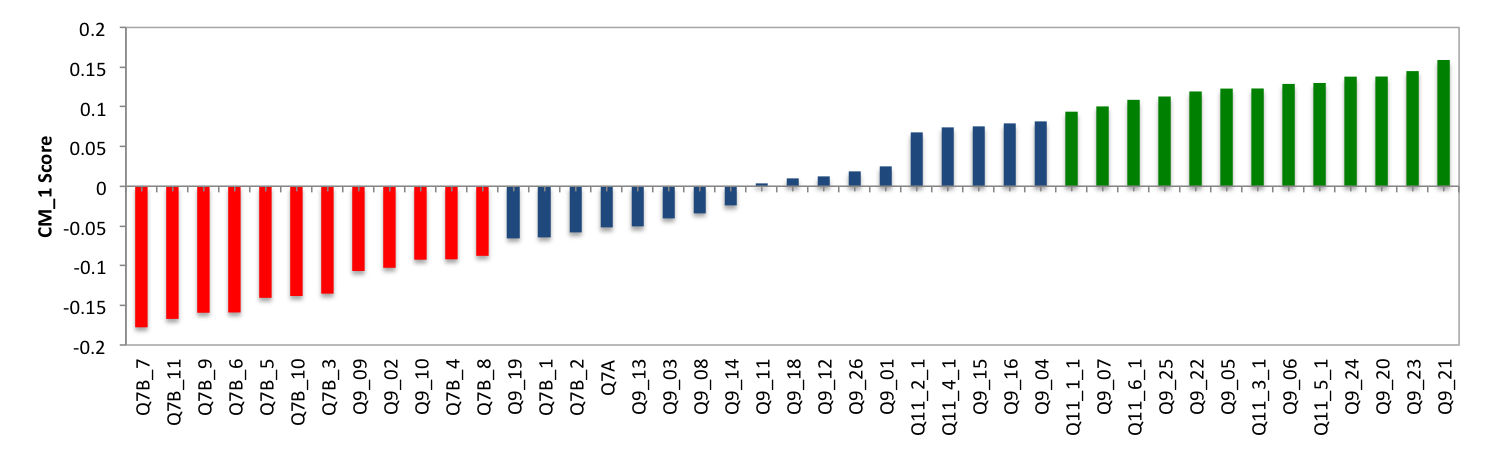
\includegraphics[ width=\textwidth ]{CM1_Cluster0.png}
	\caption{\textbf{CM1 Scores for the 43 questions for Cluster0, based on the
	clustering dataset.} The selected top and bottom questions are shown in red
	and green respectevly.}
	\label{fig:CM1Cluster0}
\end{figure}
\begin{figure}[h]
	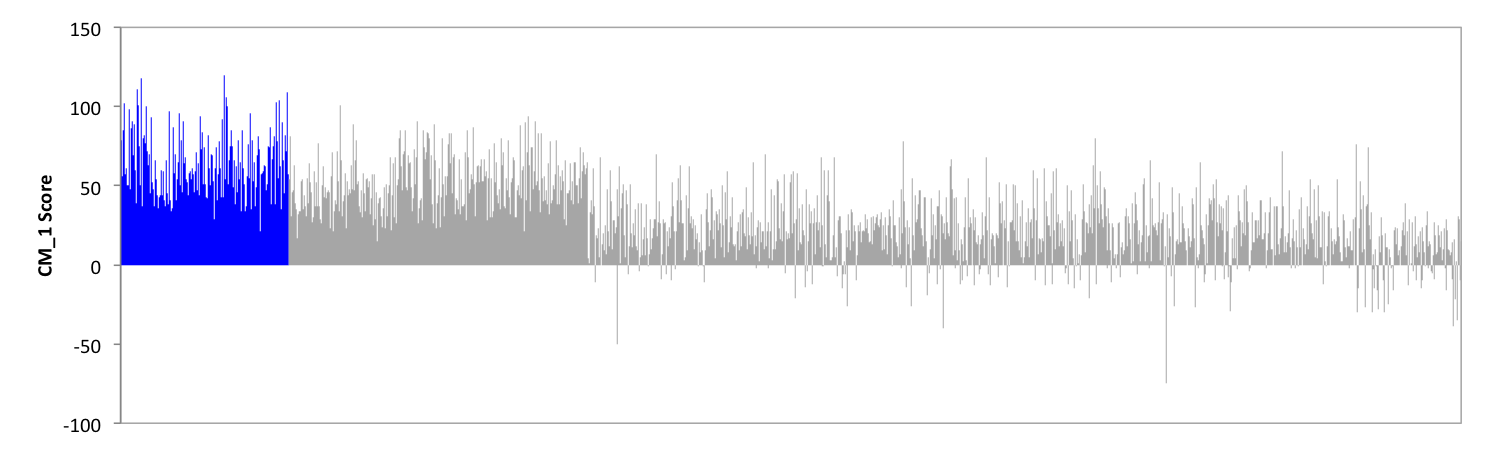
\includegraphics[ width=\textwidth]{Difference_Cluster0.png}
	\caption{\textbf{Difference between the cumulative CM1 scores for Cluster0's 12
	lowest and 13 highest scoring questions} The.}
	\label{fig:DifferencesCluster0}
\end{figure}

% Cluster 1

The Figure~\ref{fig:CM1Cluster1} demonstrate the CM1 score for the 43
questions for the Cluster0, with the 12 lowest and 11 highest ranked
questions shown in red and green respectively. The difference between the
cumulative CM1 scores for Cluster 0 is shown in the
Figure~\ref{fig:DifferencesCluster1}


\begin{figure}[h]
	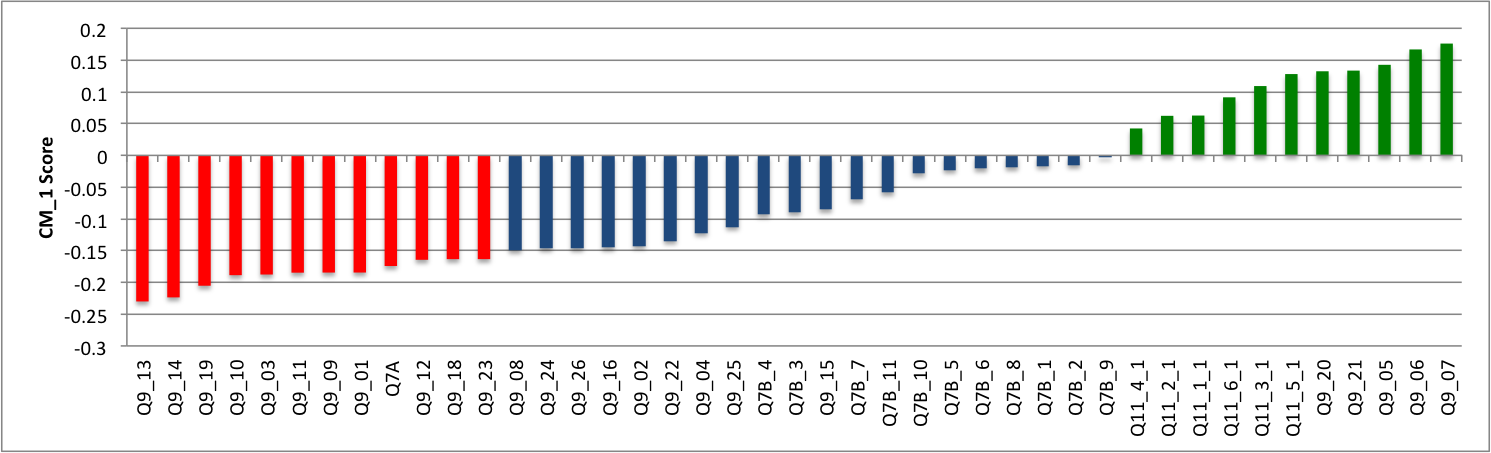
\includegraphics[ width=\textwidth ]{CM1_Cluster1.png}
	\caption{\textbf{CM1 Scores for the 43 questions for Cluster1, based on the
	clustering dataset.} The selected top and bottom questions are shown in red
	and green respectevly.}
	\label{fig:CM1Cluster1}
\end{figure}
\begin{figure}[h]
	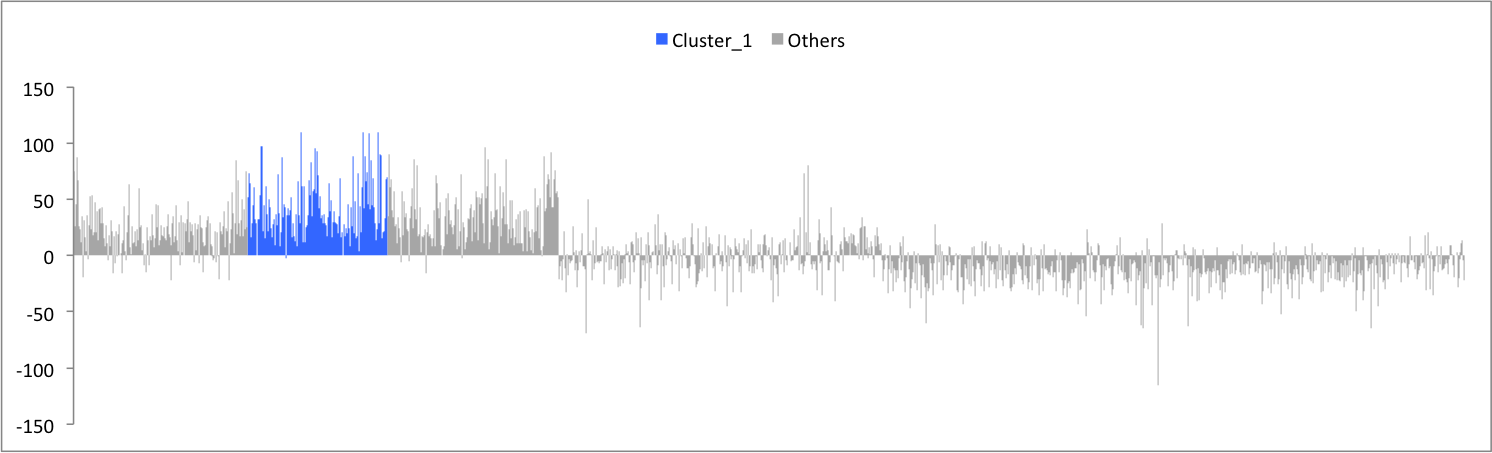
\includegraphics[ width=\textwidth]{Difference_Cluster1.png}
	\caption{\textbf{Difference between the cumulative CM1 scores for Cluster1's 12
	lowest and 13 highest scoring questions} The.}
	\label{fig:DifferencesCluster1}
\end{figure}

% Cluster 2

\begin{figure}[h]
	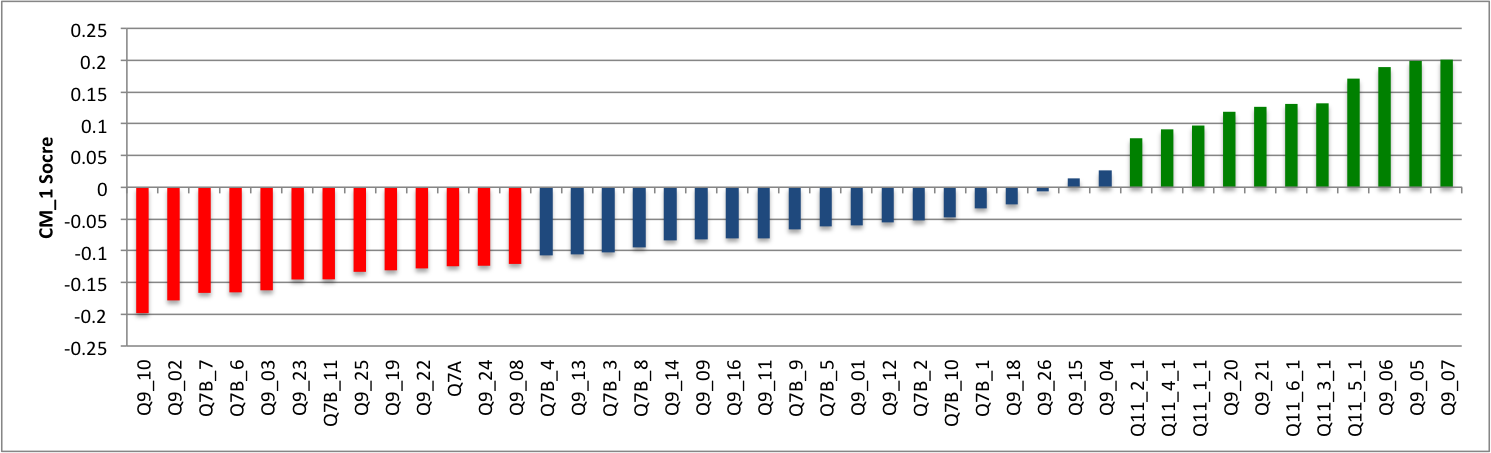
\includegraphics[ width=\textwidth ]{CM1_Cluster2.png}
	\caption{\textbf{CM1 Scores for the 43 questions for Cluster2, based on the
	clustering dataset.} The selected top and bottom questions are shown in red
	and green respectively.}
	\label{fig:CM1Cluster2}
\end{figure}
\begin{figure}[h]
	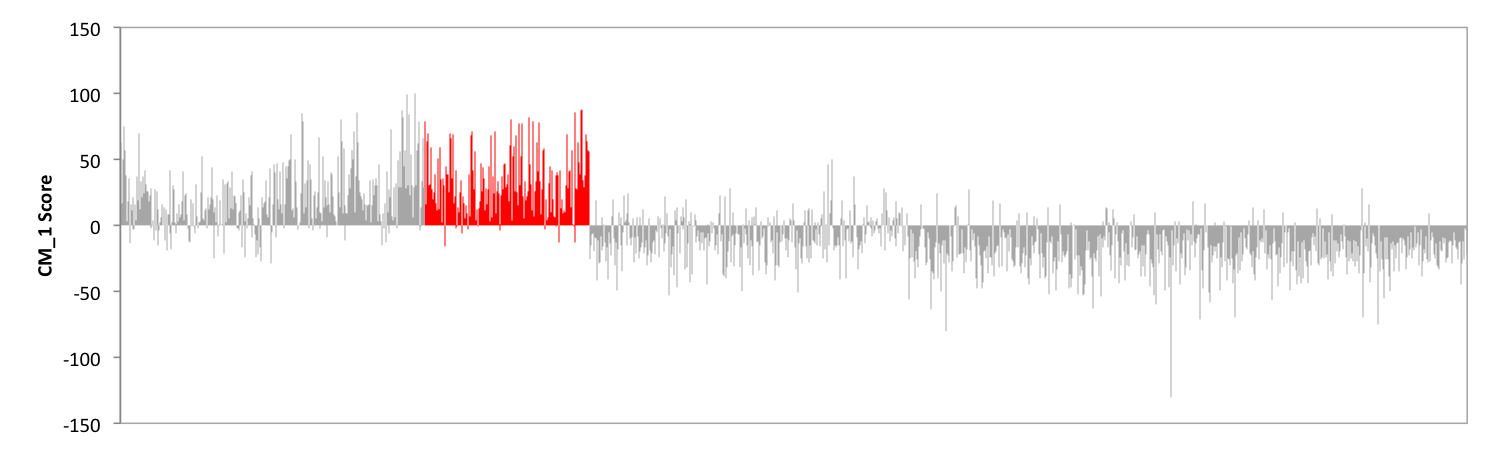
\includegraphics[ width=\textwidth]{Difference_Cluster2.png}
	\caption{\textbf{Difference between the cumulative CM1 scores for Cluster2's 12
	lowest and 13 highest scoring questions} The.}
	\label{fig:DifferencesCluster2}
\end{figure}

% Cluster 3

\begin{figure}[h]
	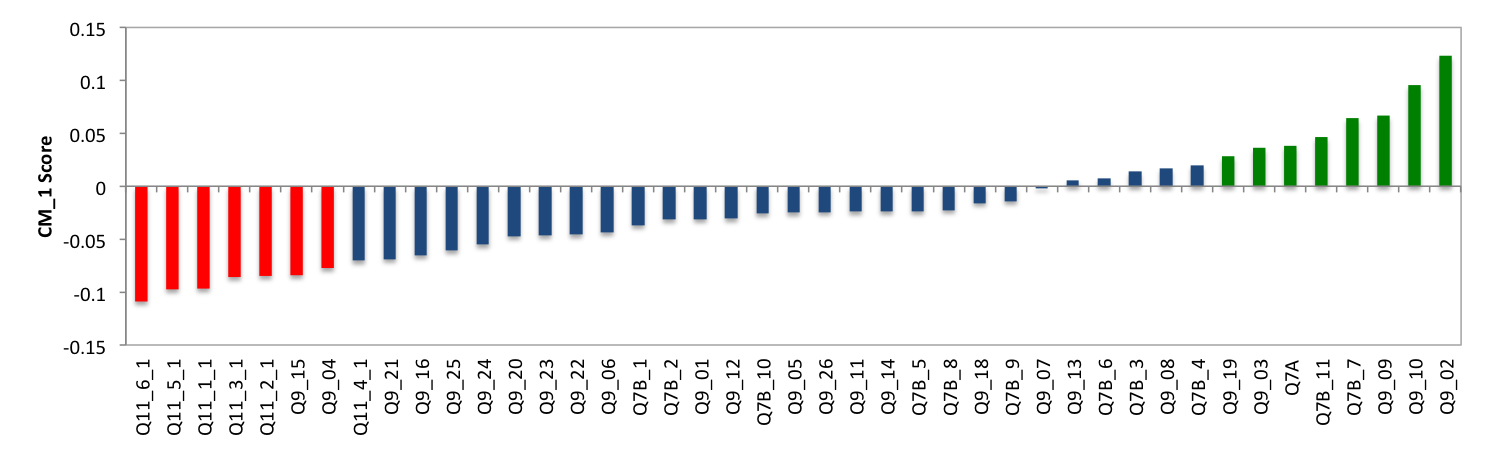
\includegraphics[ width=\textwidth ]{CM1_Cluster3.png}
	\caption{\textbf{CM1 Scores for the 43 questions for Cluster3, based on the
	clustering dataset.} The selected top and bottom questions are shown in red
	and green respectively.}
	\label{fig:CM1Cluster3}
\end{figure}
\begin{figure}[h]
	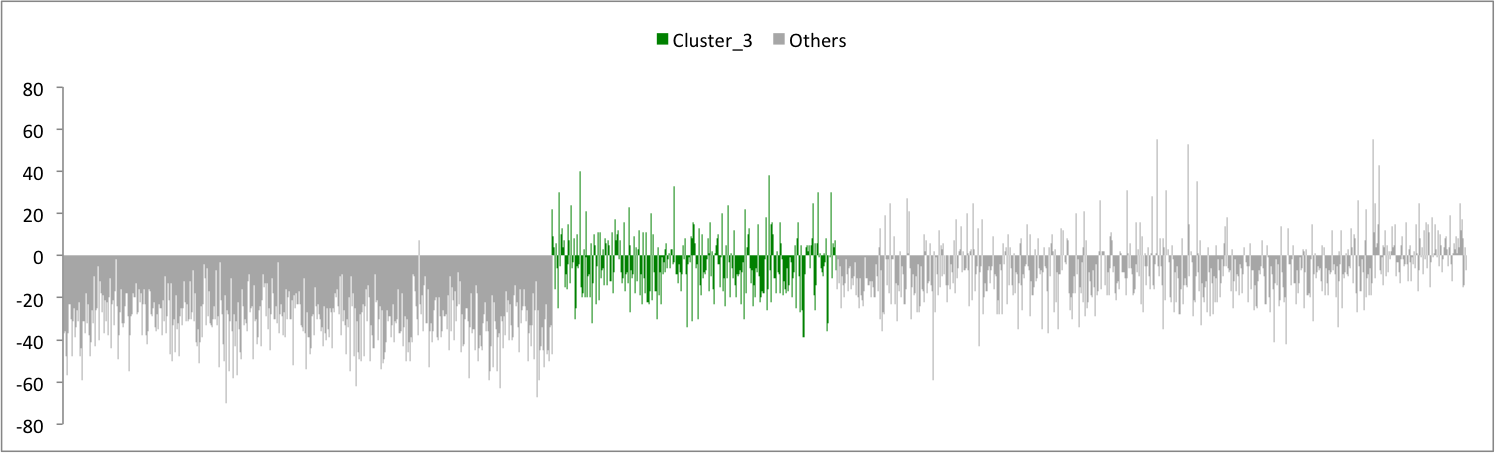
\includegraphics[ width=\textwidth]{Difference_Cluster3.png}
	\caption{\textbf{Difference between the cumulative CM1 scores for Cluster3's 12
	lowest and 13 highest scoring questions} The.}
	\label{fig:DifferencesCluster3}
\end{figure}

% Cluster 4

\begin{figure}[h]
	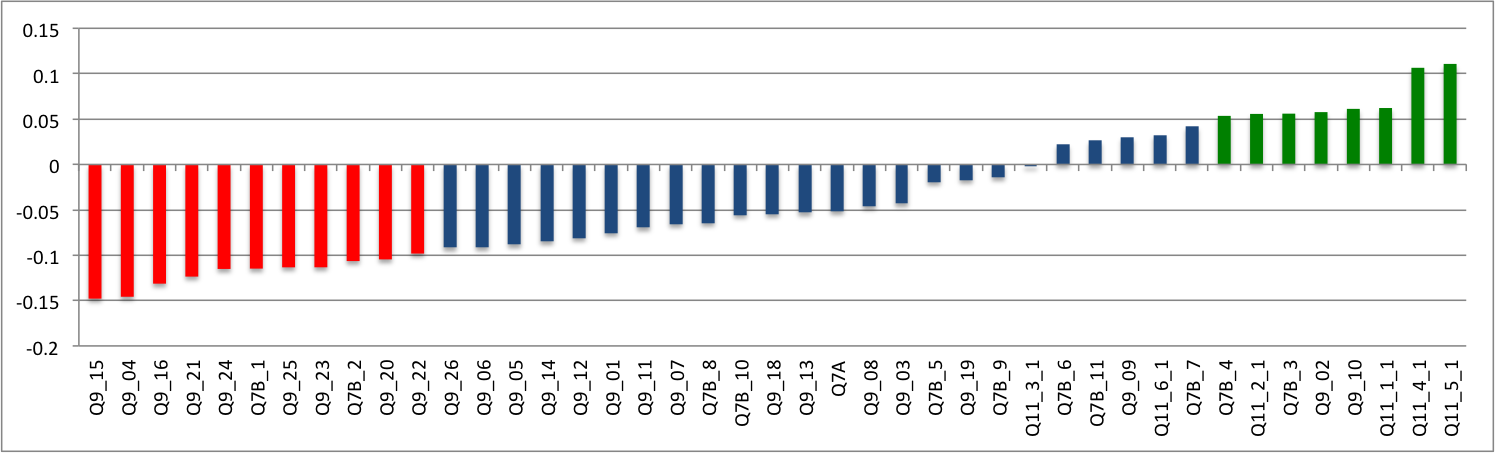
\includegraphics[ width=\textwidth ]{CM1_Cluster4.png}
	\caption{\textbf{CM1 Scores for the 43 questions for Cluster4, based on the
	clustering dataset.} The selected top and bottom questions are shown in red
	and green respectively.}
	\label{fig:CM1Cluster4}
\end{figure}
\begin{figure}[h]
	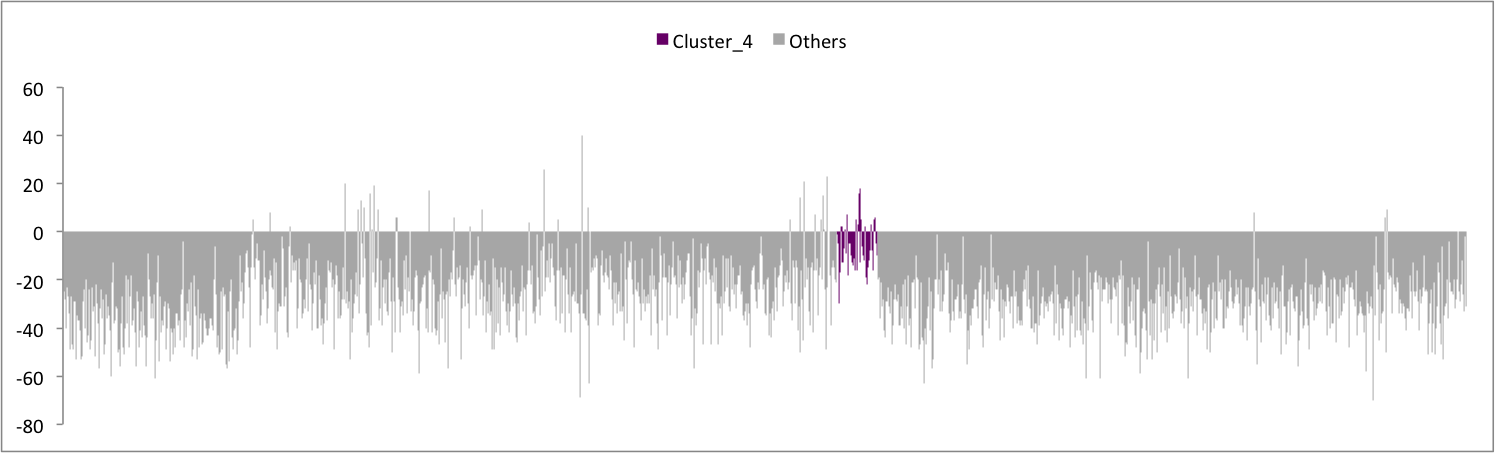
\includegraphics[ width=\textwidth]{Difference_Cluster4.png}
	\caption{\textbf{Difference between the cumulative CM1 scores for Cluster4's 12
	lowest and 13 highest scoring questions} The.}
	\label{fig:DifferencesCluster4}
\end{figure}

% Cluster 5

\begin{figure}[h]
	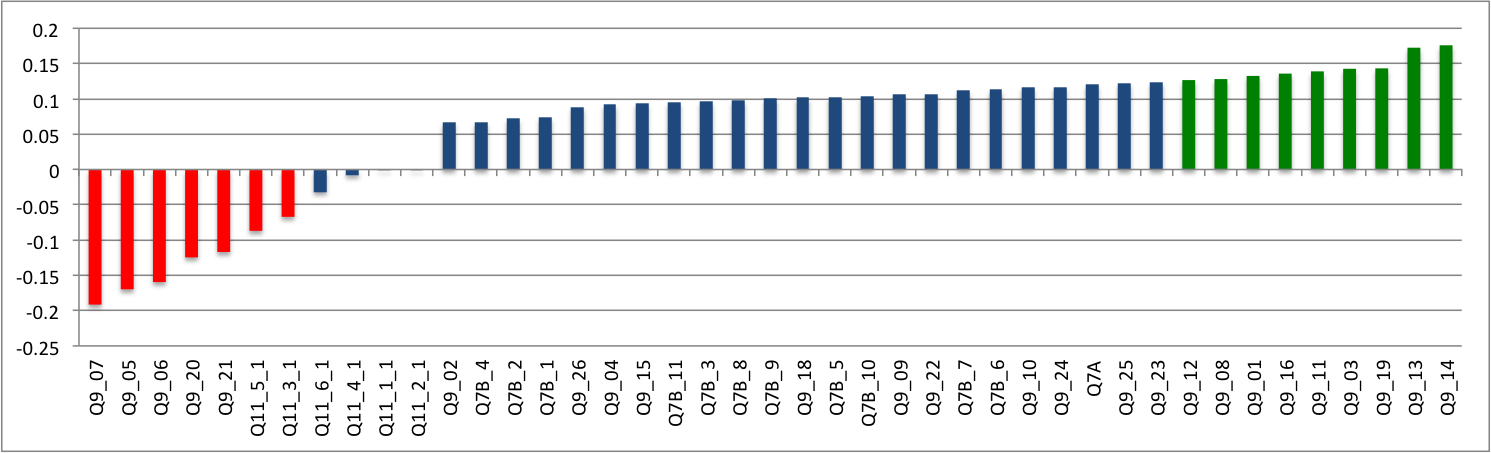
\includegraphics[ width=\textwidth ]{CM1_Cluster5.png}
	\caption{\textbf{CM1 Scores for the 43 questions for Cluster5, based on the
	clustering dataset.} The selected top and bottom questions are shown in red
	and green respectively.}
	\label{fig:CM1Cluster5}
\end{figure}
\begin{figure}[h]
	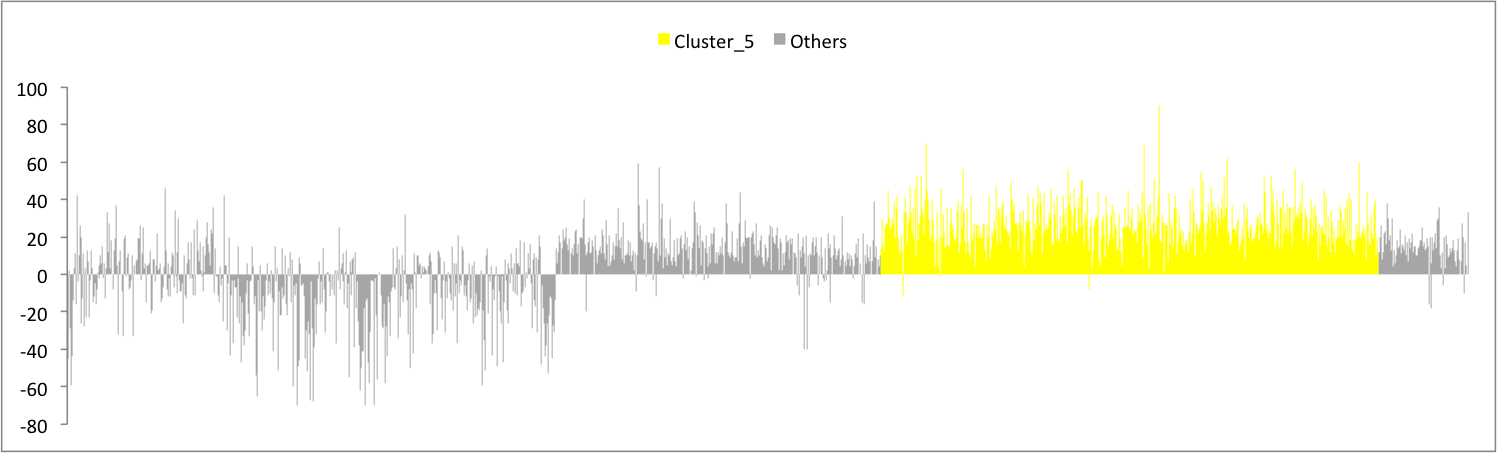
\includegraphics[ width=\textwidth]{Difference_Cluster5.png}
	\caption{\textbf{Difference between the cumulative CM1 scores for Cluster5's 12
	lowest and 13 highest scoring questions} The.}
	\label{fig:DifferencesCluster5}
\end{figure}

% Cluster 6

\begin{figure}[h]
	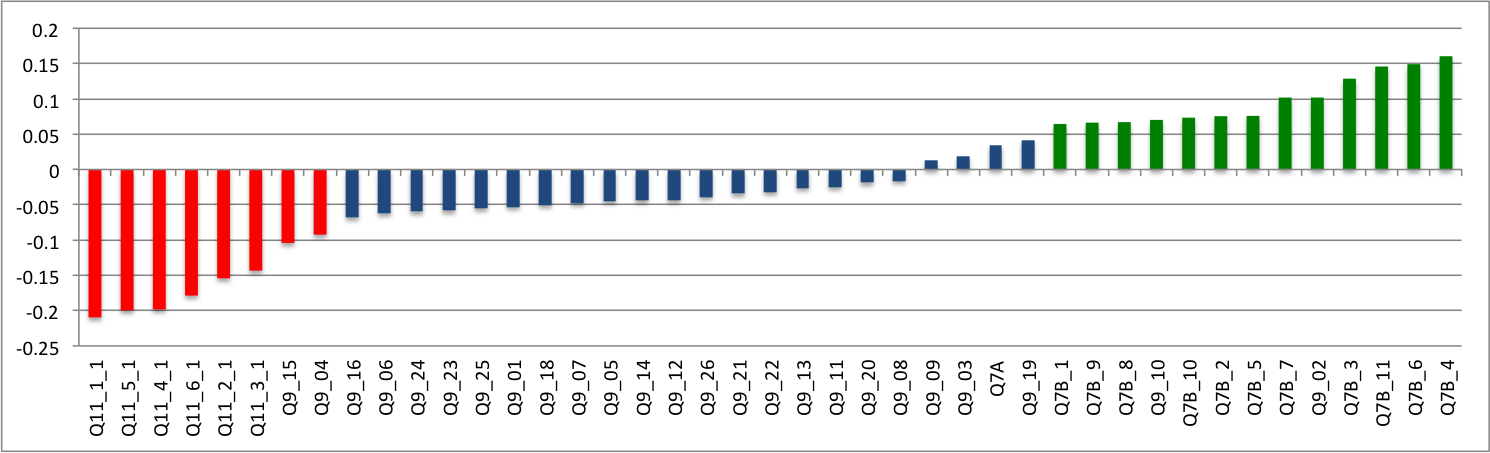
\includegraphics[ width=\textwidth ]{CM1_Cluster6.png}
	\caption{\textbf{CM1 Scores for the 43 questions for Cluster6, based on the
	clustering dataset.} The selected top and bottom questions are shown in red
	and green respectevly.}
	\label{fig:CM1Cluster6}
\end{figure}
\begin{figure}[h]
	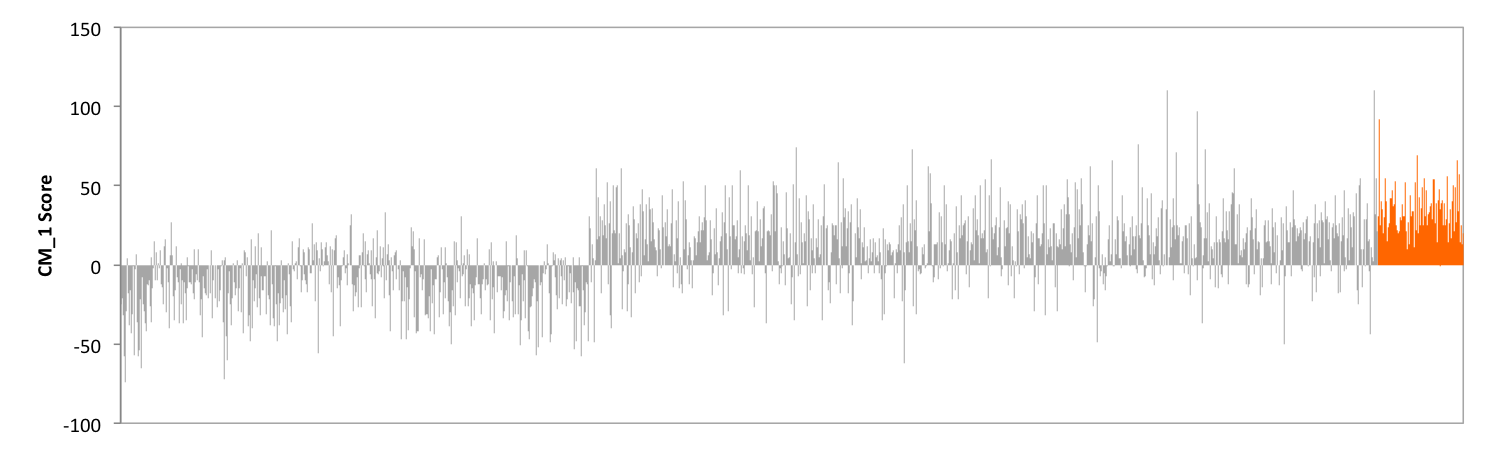
\includegraphics[ width=\textwidth]{Difference_Cluster6.png}
	\caption{\textbf{Difference between the cumulative CM1 scores for Cluster6's 12
	lowest and 13 highest scoring questions} The.}
	\label{fig:DifferencesCluster6}
\end{figure}


\subsubsection{Description of Clusters}




\subsection{Discussion and Conclusion}
%(together)

\bibliography{references}

\end{document}



